%----------------------------------------------------------------------------------------
%	PACKAGES AND OTHER DOCUMENT CONFIGURATIONS
%----------------------------------------------------------------------------------------
\documentclass[12pt]{article}
\usepackage{graphicx}
\usepackage{amsmath,amsfonts,stmaryrd,amssymb} % Math packages
\usepackage{bm}
\usepackage{steinmetz}
\usepackage{enumitem}
\graphicspath{{images/}}
\usepackage{float}
\usepackage{hyperref}
\hypersetup{
	colorlinks=true,
	linkcolor=blue,
	filecolor=magenta,      
	urlcolor=cyan,
	pdftitle={Overleaf Example},
	pdfpagemode=FullScreen,
}
\urlstyle{same}
\usepackage{mathtools}
\usepackage{fancyhdr}
\usepackage{xcolor}
\usepackage[american,RPvoltages]{circuiTikz}
\usepackage{tikz, tikz-cd}
\usepackage{pgfplots}
\usepackage{siunitx}
\usetikzlibrary{spy,shapes,arrows, arrows.meta, bending, decorations.markings}
\pgfplotsset{width=10cm,compat=1.18}
\usepackage{lmodern} % package for changing font size
\usepackage{lastpage}
\renewcommand{\figurename}{Figura}
\usepackage{tcolorbox}
\usepackage{lipsum}
%\usepackage{enumerate} % Custom item numbers for enumerations
\usepackage[ruled]{algorithm2e} % Algorithms
\usepackage[framemethod=tikz]{mdframed} % Allows defining custom boxed/framed environments
\usepackage{listings} % File listings, with syntax highlighting
%\lstset{basicstyle=\ttfamily,} % Typeset listings in monospace font
\usepackage{lipsum}
\tcbuselibrary{listings,theorems,skins,vignette,raster,breakable,magazine,poster,fitting,hooks}
\usepackage[T1]{fontenc}
\usepackage{tgbonum}
 \fontfamily{garamond}
\definecolor{myblue}{RGB}{24, 51, 73}
%----------------------------------------------------------------------------------------
%	DOCUMENT MARGINS
%----------------------------------------------------------------------------------------

\usepackage{geometry} % Required for adjusting page dimensions and margins
\geometry{
	paper=a4paper, % Paper size, change to letterpaper for US letter size
	top=2.5cm, % Top margin
	bottom=3cm, % Bottom margin
	left=2cm, % Left margin
	right=2.5cm, % Right margin
	headheight=14pt, % Header height
	footskip=1.5cm, % Space from the bottom margin to the baseline of the footer
	headsep=1.2cm, % Space from the top margin to the baseline of the header
	%showframe, % Uncomment to show how the type block is set on the page
}

%----------------------------------------------------------------------------------------
%	FONTS
%----------------------------------------------------------------------------------------

\usepackage[utf8]{inputenc} % Required for inputting international characters
\usepackage[T1]{fontenc} % Output font encoding for international characters
\usepackage{XCharter} % Use the XCharter fonts
\usepackage{tgbonum}

\makeatletter
\pgfcircdeclarebipole{}{\ctikzvalof{bipoles/vsourcesin/height}}{sVpm}{\ctikzvalof{bipoles/vsourcesin/height}}{\ctikzvalof{bipoles/vsourcesin/width}}{
	
	\pgfsetlinewidth{\pgfkeysvalueof{/tikz/circuitikz/bipoles/thickness}\pgfstartlinewidth}
	\pgfpathellipse{\pgfpointorigin}{\pgfpoint{0}{\pgf@circ@res@up}}{\pgfpoint{\pgf@circ@res@left}{0}}
	\pgfusepath{draw}     
	\pgftext[bottom,rotate=90,y=\ctikzvalof{bipoles/vsourceam/margin}\pgf@circ@res@down]{\scriptsize$-$}
	\pgftext[top,rotate=90,y=\ctikzvalof{bipoles/vsourceam/margin}\pgf@circ@res@up]{\scriptsize$+$}
	
	\pgf@circ@res@up = .35\pgf@circ@res@up
	\pgfscope
	\pgftransformrotate{90}
	\pgfpathmoveto{\pgfpoint{-\pgf@circ@res@up}{0cm}}
	\pgfpathsine{\pgfpoint{.5\pgf@circ@res@up}{.4\pgf@circ@res@up}}
	\pgfpathcosine{\pgfpoint{.5\pgf@circ@res@up}{-.4\pgf@circ@res@up}}
	\pgfpathsine{\pgfpoint{.5\pgf@circ@res@up}{-.4\pgf@circ@res@up}}
	\pgfpathcosine{\pgfpoint{.5\pgf@circ@res@up}{.4\pgf@circ@res@up}}
	\pgfusepath{draw}
	\endpgfscope
}
\def\pgf@circ@sVpm@path#1{\pgf@circ@bipole@path{sVpm}{#1}}
\compattikzset{sinusoidal voltage source pm/.style = {\circuitikzbasekey, /tikz/to path=\pgf@circ@sVpm@path, \circuitikzbasekey/bipole/is voltage=true, \circuitikzbasekey/bipole/is voltageoutsideofsymbol=true, v=#1 }}
\compattikzset{sVpm/.style = {\comnpatname sinusoidal voltage source pm = #1}}

\pgfcircdeclarebipole{}{\ctikzvalof{bipoles/vsourcesin/height}}{sVpmh}{\ctikzvalof{bipoles/vsourcesin/height}}{\ctikzvalof{bipoles/vsourcesin/width}}{
	
	\pgfsetlinewidth{\pgfkeysvalueof{/tikz/circuitikz/bipoles/thickness}\pgfstartlinewidth}
	\pgfpathellipse{\pgfpointorigin}{\pgfpoint{0}{\pgf@circ@res@up}}{\pgfpoint{\pgf@circ@res@left}{0}}
	\pgfusepath{draw}     
	\pgftext[center,x=0.2\pgf@circ@res@down-\ctikzvalof{bipoles/vsourceam/margin}\pgf@circ@res@down]{\scriptsize$-$}
	\pgftext[top,rotate=90,y=\ctikzvalof{bipoles/vsourceam/margin}\pgf@circ@res@up]{\scriptsize$+$}
	
	\pgf@circ@res@up = .35\pgf@circ@res@up
	\pgfscope
	\pgftransformrotate{90}
	\pgfpathmoveto{\pgfpoint{-\pgf@circ@res@up}{0cm}}
	\pgfpathsine{\pgfpoint{.5\pgf@circ@res@up}{.4\pgf@circ@res@up}}
	\pgfpathcosine{\pgfpoint{.5\pgf@circ@res@up}{-.4\pgf@circ@res@up}}
	\pgfpathsine{\pgfpoint{.5\pgf@circ@res@up}{-.4\pgf@circ@res@up}}
	\pgfpathcosine{\pgfpoint{.5\pgf@circ@res@up}{.4\pgf@circ@res@up}}
	\pgfusepath{draw}
	\endpgfscope
}
\def\pgf@circ@sVpmh@path#1{\pgf@circ@bipole@path{sVpmh}{#1}}
\compattikzset{sinusoidal voltage source pmh/.style = {\circuitikzbasekey, /tikz/to path=\pgf@circ@sVpmh@path, \circuitikzbasekey/bipole/is voltage=true, \circuitikzbasekey/bipole/is voltageoutsideofsymbol=true, v=#1 }}
\compattikzset{sVpmh/.style = {\comnpatname sinusoidal voltage source pmh = #1}}
\makeatother


%----------------------------------------------------------------------------------------
%	BEGIN DOCUMENT
%----------------------------------------------------------------------------------------

\begin{document}
	%\thispagestyle{empty}
	\begin{tikzpicture}[remember picture, overlay]
		\node[anchor=north west, inner sep=0pt] at (current page.north west) {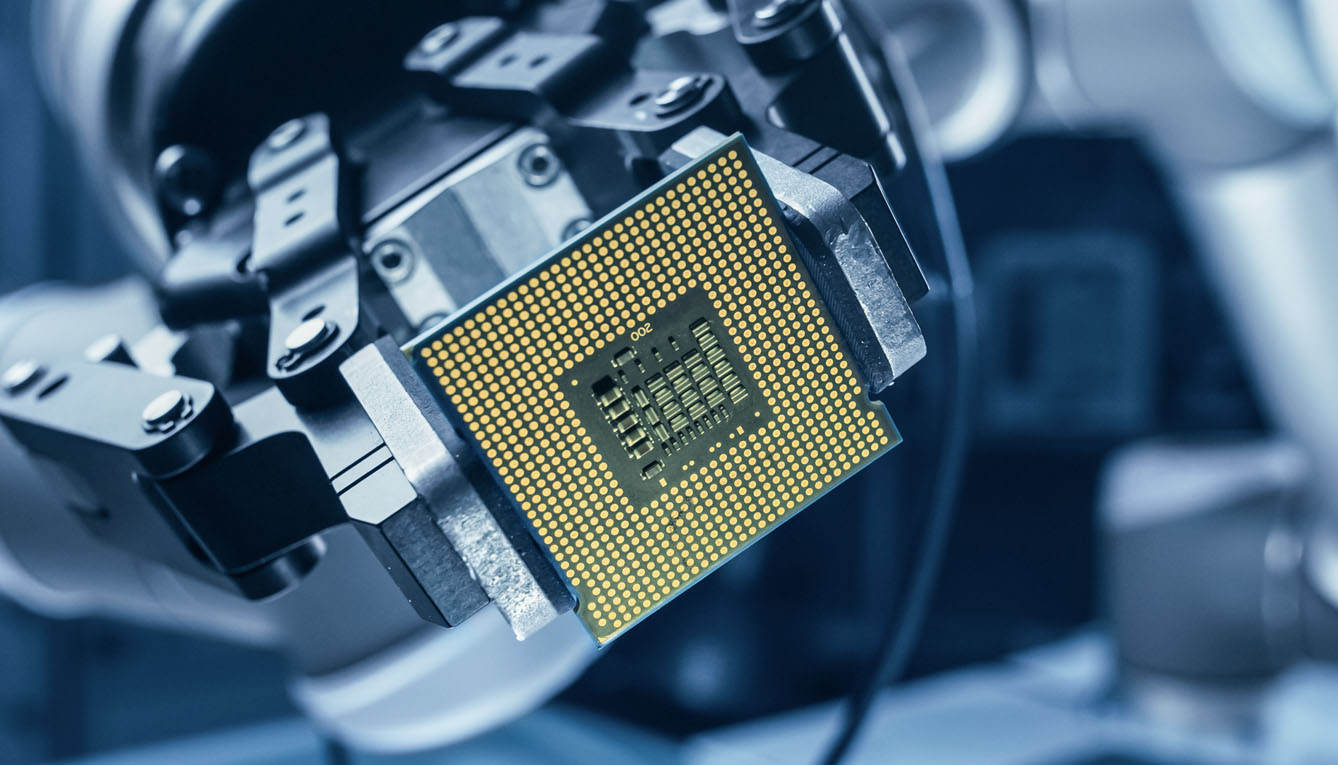
\includegraphics[width=\paperwidth, height=.5\paperheight]{picture1}};
	\end{tikzpicture}

	\vspace{13cm}
	\noindent \textcolor{myblue}{\fontsize{40pt}{40pt}\selectfont \textbf{Amplificador Multietapa}}\\\\\\
	{\fontsize{18pt}{18pt}\selectfont Julio, 2023} 
	
	\newpage
	\section*{Amplificador Multietapa}
	El amplificador de la figura 1 consiste de dos amplificadores en emisor común idénticos conectados en cascada. Observe que la resistencia de entrada de la segunda etapa $R_{in2}$ constituye la resistencia de carga de la primera etapa. Encuentre $R_{in_1}$, $v_{b_1}/v_{sig}$, $R_{in_2}$, $v_{b_2}/v_{b_1}$, $v_o/v_{b_2}$ y $v_o/v_{sig}$.
	
	
	\begin{figure}[H]
		%\centering	
		\begin{tikzpicture}[scale=0.7]
			\draw (0,0) node[ground]{} to[V, l=$v_{sig}$] (0,4) 
						to[R, l=$R_{sig}$] ++(3,0)
						to[C, l=$\texttt{Inf}$] ++(2,0) coordinate(node1)
						to[R, l=$R_{B2}$, *-] ++(0,-4) node[ground]{};
			\draw (node1) to[R, l=$R_{B1}$] ++(0,4) node[vcc]{$V_{CC}$};
			\draw (node1) to[short] ++(2,0) coordinate(node2);
			\draw (node2) node[npn, right](Q1){};
			\draw (Q1.C) to[R, l=$R_{C1}$] ++(0,3.25) node[vcc]{$V_{CC}$};
			\draw (Q1.E) to[R, l=$R_{E1}$] ++(0,-3) node[ground]{};
			\draw (Q1.E) to[short, *-] ++(2,0)
						 to[C, l=$\texttt{Inf}$] ++(0,-3) node[ground]{};
			\draw (Q1.C) to[C, l=$\texttt{Inf}$, *-] ++(3,0)
						 to[short] ++(0,-0.95)
						 to[short] ++(2,0) coordinate(node3);
			\draw (node3) to[R, l=$R_{B3}$, *-] ++(0,4) node[vcc]{$V_{CC}$};
			\draw (node3) to[R, l=$R_{B4}$] ++(0,-4) node[ground]{};
			\draw (node3) to[short] ++(2,0) coordinate(node4);
			\draw (node4) node[npn, right](Q2){};
			\draw (Q2.C) to[R, l=$R_{C2}$, *-] ++(0,3.25) node[vcc]{$V_{CC}$};
			\draw (Q2.E) to[R, l=$R_{E2}$] ++(0,-3) node[ground]{};
			\draw (Q2.E) to[short, *-] ++(2,0)
						 to[C, l=$\texttt{Inf}$] ++(0,-3) node[ground]{};
			\draw (Q2.C) to[short] ++(2,0)
						 to[C, l=$\texttt{Inf}$] ++(2,0)
						 to[R, l=$R_L$] ++(0,-5) node[ground]{};
			\draw [cyan, densely dashed] (3,10) -- (3,-2);
			\draw (1,10) node[cyan]{$\texttt{Fuente}$};
			\draw [cyan, densely dashed] (11.5,10) -- (11.5,-2);
			\draw (7, 10) node[cyan]{$\texttt{Etapa 1}$};
			\draw [cyan, densely dashed] (18.5,10) -- (18.5,-2);
			\draw (15, 10) node[cyan]{$\texttt{Etapa 2}$};
			\draw (20, 10) node[cyan]{$\texttt{Carga}$};
		\end{tikzpicture}
		\caption{Amplificador multietapa}	
		\label{fig:figura1}
	\end{figure}
	
	\noindent Determinamos el equivalente en pequeña señal eliminando las fuentes de cd y reempazando los transistores por su equivalente híbrido $\pi$ según se indica en la figura 2.
	
	\begin{figure}[H]
		%\centering	
		\begin{tikzpicture}[scale=0.7]
			\draw (0,0) to[sVpm, invert] ++(0,4)
						to[R, l=$R_{sig}$] ++(3,0) coordinate(nodeA)
						to[R, l_=$R_{eq_1}$] ++(0,-4)
						to[short] ++(-3,0);
			\draw (nodeA) to[short, *-] ++(2,0)
						to[R, l=$r_{\pi_1}$, v=$v_{\pi_1}$] ++(0,-4) coordinate(nodeB)
						to[short, -*] ++(-2,0);			
			\draw (nodeB) to[short, *-*] ++(4,0)
						to[cI, invert, l=$g_{m_1} V_{\pi_1}$] ++(0,4)
						to[short] ++(2,0) coordinate(nodeC)
						to[R, l_=$R_{C1}$] ++(0,-4)
						to[short] ++(-2,0);
			\draw (nodeC) to[short, *-] ++(2,0) coordinate(nodeD)
						to[R, l_=$R_{eq_2}$] ++(0,-4)
						to[short, -*] ++(-2,0);
			\draw (nodeD) to[short, *-] ++(2,0)
						to[R, l=$r_{\pi_2}$, v=$v_{\pi 2}$] ++(0,-4) coordinate(nodeE)
						to[short, -*] ++(-2,0);
			\draw (nodeE) to[short] ++(4,0)
						to[cI, invert, l=$g_{m_2} v_{\pi 2}$] ++(0,4)
						to[short] ++(2,0) coordinate(nodeF)
						to[R, l=$R_{C_2}$] ++(0,-4)
						to[short, -*] ++(-2,0);
			\draw (nodeF) to[short, *-] ++(2,0)
						to[R, l=$R_L$] ++(0,-4)
						to[short, -*] ++(-2,0);
			\draw (nodeF) node[above]{$v_o$};
 		\end{tikzpicture}
		\caption{Circuito equivalente en pequeña señal}	
		\label{fig:figura2}
	\end{figure}
	
	\section*{Determinando la resistencia de entrada $R_{in_1}$}
	Para determinar la resistencia de entrada $R_{in_1}$ se conecta una fuente de voltaje $V_x$ en paralelo con las resistencias $R_B$ y $r_{\pi_1}$. El circuito se muestra en la figura 3.
	
	\begin{figure}[H]
		%\centering	
		\begin{tikzpicture}[scale=0.7]
			\draw (0,0) to[V, l=$V_X$] ++(0,4)
			to[short, f=$I_X$] ++(3,0) coordinate(vx)
			to[R, l_=$R_{eq_1}$, f>_=$I_1$] ++(0,-4)
			to[short] ++(-3,0);
			\draw (vx) node[above]{$V_X$};
			\draw (nodeA) to[short, *-] ++(2,0)
			to[R, l=$r_{\pi_1}$, v=$v_{\pi_1}$, f>^=$I_2$] ++(0,-4) coordinate(nodeB)
			to[short, -*] ++(-2,0);			
			\draw (nodeB) to[short, *-*] ++(4,0)
			to[cI, invert, l=$g_{m_1} V_{\pi_1}$] ++(0,4)
			to[short] ++(2,0) coordinate(nodeC)
			to[R, l_=$R_{C1}$] ++(0,-4)
			to[short] ++(-2,0);
			\draw (nodeC) to[short, *-] ++(2,0) coordinate(nodeD)
			to[R, l_=$R_{eq_2}$] ++(0,-4)
			to[short, -*] ++(-2,0);
			\draw (nodeD) to[short, *-] ++(2,0)
			to[R, l=$r_{\pi_2}$, v=$v_{\pi 2}$] ++(0,-4) coordinate(nodeE)
			to[short, -*] ++(-2,0);
			\draw (nodeE) to[short] ++(4,0)
			to[cI, invert, l=$g_{m_2} v_{\pi 2}$] ++(0,4)
			to[short] ++(2,0) coordinate(nodeF)
			to[R, l=$R_{C_2}$] ++(0,-4)
			to[short, -*] ++(-2,0);
			\draw (nodeF) to[short, *-] ++(2,0)
			to[R, l=$R_L$] ++(0,-4)
			to[short, -*] ++(-2,0);
			\draw (nodeF) node[above]{$v_o$};
		\end{tikzpicture}
		\caption{Obteniendo la resistencia de entrada}	
		\label{fig:figura3}
	\end{figure}
	
	
	\noindent Evaluando la LCK en el nodo $V_X$ en el circuito de la figura 3 obtenemos
	\begin{align}
		I_X = I_1 + I_2\nonumber
	\end{align}
	
	\noindent O bien
	\begin{align}
		I_X &= \frac{V_X}{R_{eq_1}} + \frac{V_X}{r_{\pi_1}}\nonumber\\
		I_X &= \left( \frac{1}{R_{eq_1}} + \frac{1}{r_{\pi_1}} \right)V_X\nonumber
	\end{align}
	
	\noindent Por lo tanto
	\begin{tcolorbox}[colback=red!5!white,colframe=red!75!black,arc=0mm,boxrule=0mm,width=(\linewidth+0.5cm)]
		\begin{equation}
			R_{in_1} = \frac{V_X}{I_X} = \frac{1}{ \frac{1}{R_{eq_q}} + \frac{1}{r_{\pi_1}} } = R_{eq_1} \parallel r_{\pi_1}
		\end{equation}
	\end{tcolorbox}
	
	\section*{Determinando $v_{b_1}/v_{sig}$}
	Para determinar la primer ganancia $v_{b_1}/v_{sig}$ aplicamos la regla de división de tensión en la primera sección del circuito de la figura 2
	
	\begin{align*}
		v_{b_1} = \frac{R_{eq_1} || r_{\pi_1}}{R_{sig} + R_{eq_1} || r_{\pi_1}} v_{sig}
	\end{align*}
	
	\noindent O bien
	\begin{tcolorbox}[colback=red!5!white,colframe=red!75!black,arc=0mm,boxrule=0mm,width=(\linewidth+0.5cm)]
		\begin{equation}
			\frac{v_{b_1}}{v_{sig}} = \frac{R_{eq_1} || r_{\pi_1}}{R_{sig} + R_{eq_1} || r_{\pi_1}} v_{sig}
		\end{equation}
	\end{tcolorbox}
	
	\section*{Determinando $R_{in_2}$}
	Para determinar la resistencia de entrada $R_{in_2}$ observe el circuito de la figura 4
	\begin{figure}[H]
		\centering	
		\begin{tikzpicture}[scale=0.7]
			\draw (0,0)   to[sVpm, invert, l=$V_X$] ++(0,4)
						  to[short, -*, f=$I_X$] ++(3,0) coordinate(nodeA)
						  to[R, l=$R_{B2}$, f>_=$I_1$, -*] ++(0,-4)
						  to[short] ++(-3,0);
			\draw (nodeA) to[short] ++(3,0)
						  to[R, l=$r_{\pi_2}$, v=$v_{\pi_2}$, f>^=$I_2$] ++(0,-4) coordinate(nodeB)
						  to[short] ++(-3,0);
			\draw (nodeB) to[short, *-*] ++(5,0) coordinate(nodeD)
						  to[cI, invert, l=$g_{m_2} v_{\pi_2}$] ++(0,4)
						  to[short] ++(3,0) coordinate(nodeC)
						  to[R, l=$R_{C_2}$] ++(0,-4)
						  to[short] ++(-3,0);
			\draw (nodeC) to[short, *-] ++(3,0)
						  to[R, l=$R_L$] ++(0,-4)
						  to[short, -*] ++(-3,0);
			\coordinate (M) at ($(nodeB)!0.5!(nodeD)$);
			\draw (M) to[short, *-] (M);
			\draw (M) node[ground]{};
			\draw (nodeA) node[above]{$V_X$};
		\end{tikzpicture}
		\caption{Obteniendo la resistencia de entrada}	
		\label{fig:figura4}
	\end{figure}
	
	Realizamos exactamente los mismos pasos que hicimos para determinar la reisstencia de entrada $R_{in_1}$, es decir
	\begin{align*}
, 		I_X = I_1 + I_2
	\end{align*}
	
	\noindent Por lo tanto
	\begin{tcolorbox}[colback=red!5!white,colframe=red!75!black,arc=0mm,boxrule=0mm,width=(\linewidth+0.5cm)]
		\begin{equation}
			R_{in_2} = \frac{V_X}{I_X} = \frac{1}{ \frac{1}{R_{eq_2}} + \frac{1}{r_{\pi_2}} } = R_{eq_2} \parallel r_{\pi_2}
		\end{equation}
	\end{tcolorbox}
	
	\section*{Determinando $v_{b_2}/v_{b_1}$}
	Para determinar la ganancia $v_{b_2}/v_{b_1}$ empleamos el circuito de la figura 2, que para mayor comodidad se reproduce nuevamente en la figura (5)
	
	\begin{figure}[H]
		%\centering	
		\begin{tikzpicture}[scale=0.7]
			\draw (0,0) to[sVpm, invert] ++(0,4)
			to[R, l=$R_{sig}$] ++(3,0) coordinate(nodeA)
			to[R, l_=$R_{eq_1}$] ++(0,-4)
			to[short] ++(-3,0);
			\draw (nodeA) to[short, *-] ++(2,0)
			to[R, l=$r_{\pi_1}$, v=$v_{\pi_1}$] ++(0,-4) coordinate(nodeB)
			to[short, -*] ++(-2,0);			
			\draw (nodeB) to[short, *-*] ++(4,0) coordinate(point1)
			to[cI, invert, l=$g_{m_1} V_{\pi_1}$] ++(0,4)
			to[short] ++(2,0) coordinate(nodeC)
			to[R, l_=$R_{C1}$] ++(0,-4)
			to[short] ++(-2,0);
			\draw (nodeC) to[short, *-] ++(2,0) coordinate(nodeD)
			to[R, l_=$R_{eq_2}$] ++(0,-4)
			to[short, -*] ++(-2,0);
			\draw (nodeD) to[short, *-] ++(2,0)
			to[R, l=$r_{\pi_2}$, v=$v_{\pi 2}$, -*] ++(0,-4) coordinate(nodeE)
			to[short, -*] ++(-2,0);
			\draw (nodeE) to[short] ++(4,0)
			to[cI, invert, l=$g_{m_2} v_{\pi 2}$] ++(0,4)
			to[short] ++(2,0) coordinate(nodeF)
			to[R, l=$R_{C_2}$] ++(0,-4)
			to[short, -*] ++(-2,0);
			\draw (nodeF) to[short, *-] ++(2,0)
			to[R, l=$R_L$] ++(0,-4)
			to[short, -*] ++(-2,0);
			\draw (nodeF) node[above]{$v_o$};
			\draw (nodeA) node[above right]{$v_{\pi_1} = v_{b_1}$};
			\draw (nodeD) node[above right]{$v_{\pi_2} = v_{b_2}$};
			\coordinate (M) at ($(point1)!0.5!(nodeE)$);
			\draw (M) node[ground]{};
			\draw (M) to[short, *-] (M);
		\end{tikzpicture}
		\caption{Circuito equivalente en pequeña señal}	
		\label{fig:figura5}
	\end{figure}
	
	\noindent El voltaje en el nodo $v_{b_2}$ es:
	\begin{align*}
		v_{b_2} = -g_{m_1}\left( R_{C_2}  \parallel R_{B_2}  \parallel r_{\pi_2} \right)v_{b_1}
	\end{align*}
	
	\noindent O bien
	\begin{tcolorbox}[colback=red!5!white,colframe=red!75!black,arc=0mm,boxrule=0mm,width=(\linewidth+0.5cm)]
		\begin{equation}
			\frac{v_{b_2}}{v_{b_1}} = -g_{m_1}\left( R_{C_2}  \parallel R_{B_2}  \parallel r_{\pi_2} \right)
		\end{equation}
	\end{tcolorbox}
	
	\section*{Determinando $v_o / v_{b_2}$}
	Del circuito de la figura 5 tenemos que:
	
	\begin{align*}
		v_o = -g_{m_2} \left( R_{C_2} \parallel R_L \right)v_{b_2}
	\end{align*} 
	
	\noindent O bien
	\begin{tcolorbox}[colback=red!5!white,colframe=red!75!black,arc=0mm,boxrule=0mm,width=(\linewidth+0.5cm)]
		\begin{equation}
			\frac{v_0}{v_{b_2}} = -g_{m_2} \left( R_{C_2} \parallel R_L \right)v_{b_2}
		\end{equation}
	\end{tcolorbox}
	
	\section*{Determinando $v_o / v_{sig}$}
	La ganancia general de voltaje del circuito de la figura 2 está dado por:
	
	\begin{align}
		\frac{v_o}{v_{sig}} = \frac{v_o}{v_{b_2}} \cdot \frac{v_{b_2}}{v_{b_1}} \cdot \frac{v_{b_1}}{v_{sig}}	
	\end{align}
	
	\noindent Así, al sustituir las ecuaciones (5), (4) y (2) en la ecuación (6) obtenemos:
	\begin{tcolorbox}[colback=red!5!white,colframe=red!75!black,arc=0mm,boxrule=0mm,width=(\linewidth+0.5cm)]
		\begin{equation}
			\frac{v_o}{v_{sig}} = g_{m_1} g_{m_2} \frac{R_{eq_1} \parallel r_{\pi_1}}{R_{sig} + R_{eq_1} \parallel r_{\pi_1}} \left( R_{C_2} \parallel R_L \right) \left( R_{C_2} \parallel R_{eq_2} \parallel r_{\pi_2} \right)
		\end{equation}
	\end{tcolorbox}
	
	\section*{Determinando $R_o$}
	Para encontrar $R_o$ sea el circuito de la figura 6
	\begin{figure}[H]
		%\centering	
		\begin{tikzpicture}[scale=0.7]
			\draw (0,0) coordinate(point0)  to[R, l=$R_{sig} \parallel R_{eq_1}$] ++(0,4)
						  to[short] ++(3,0)
						  to[R, l=$r_{\pi_1}$, v=$v_{\pi_1}$,-*] ++(0,-4) coordinate(nodeA)
						  to[short] ++(-3,0);
			\draw (nodeA) to[short] ++(4,0)
						  to[cI, invert, l=$g_{m_1} v_{\pi_1}$] ++(0,4)
						  to[short] ++(3,0)
						  to[R, l=$R_{eq_2} || R_{C_2} || r_{\pi_2}$, v=$v_{\pi_2}$, -*]  ++(0,-4) node[ground]{} coordinate(nodeB)
						  to[short, -*] ++(-3,0);
			\draw (nodeB) to[short, -*] ++(5,0)
						  to[cI, invert, l_=$g_{m_2} v_{\pi_2}$] ++(0,4)
						  to[short] ++(3,0) coordinate(nodeC)
						  to[R, l=$R_{C_2}$, f>_=$I_1$] ++(0,-4)
						  to[short, *-] ++(-3,0);
			\draw (nodeC) to[short, *-, f^<=$I_X$] ++(3,0)
						  to[sVpm, l=$V_X$] ++(0,-4) coordinate(point1)
						  to[short] ++(-3,0);
			\draw (nodeC) node[above]{$V_X$};
			\coordinate (M) at ($(point0)!0.5!(point1)$);
			%\draw (M) node[ground]{};
			%\draw (M) to[short, *-] (M);
		\end{tikzpicture}
		\caption{Circuito equivalente en pequeña señal}	
		\label{fig:figura6}
	\end{figure}
	
	\noindent Aplicamos la LKC sobre el nodo $V_X$
	\begin{align}
		I_X = I_1 + g_{m_2} v_{\pi_2}\nonumber
	\end{align}
	
	\noindent O bien
	\begin{align}
		I_X = \frac{V_X}{R_{C2}} + g_{m_2} v_{\pi_2}
	\end{align}
	
	\noindent Sin embargo
	\begin{align}
		v_{\pi_2} = -g_{m_1}\left( R_{eq_2} \parallel R_{C2} \parallel r_{\pi_2} \right)v_{\pi_1}
	\end{align}
	
	\noindent Donde
	\begin{align}
		v_{\pi_1} = 0
	\end{align}
	
	\noindent Por lo tanto
	\begin{align}
		I_X = \frac{V_X}{R_{C2}}\nonumber
	\end{align}
	
	\begin{tcolorbox}[colback=red!5!white,colframe=red!75!black,arc=0mm,boxrule=0mm,width=(\linewidth+0.5cm)]
		\begin{equation}
			R_O = \frac{V_X}{I_X} = R_{C2}
		\end{equation}
	\end{tcolorbox}
\end{document}